\documentclass{beamer}

% THEME (Metropolis)
\usetheme[numbering=counter,progressbar=foot]{metropolis} % clean + progress bar
\usepackage{appendixnumberbeamer}

% FONTS (works with pdfLaTeX; for nicer system fonts, compile with XeLaTeX)
\usepackage[T1]{fontenc}
\usepackage[utf8]{inputenc}
\usepackage{lmodern}

% MATH / GRAPHICS
\usepackage{amsmath, amssymb}
\usepackage{graphicx}
\graphicspath{{figures/}}

% BIB (optional) — comment out if not needed
\usepackage[numbers]{natbib}
\usepackage{bibentry}

\usepackage{algorithm, algpseudocode}
\usepackage{float}

\usepackage{listings}
\usepackage{booktabs}        % for \toprule \midrule \bottomrule
\usepackage{xcolor} % for colors
\usepackage{adjustbox} % to scale only if needed
\definecolor{codebg}{RGB}{245,247,250}
\definecolor{codekw}{RGB}{0,90,160}
\definecolor{codecm}{RGB}{110,110,110}
\definecolor{codestr}{RGB}{160,60,60}
\definecolor{codenum}{RGB}{120,120,120}

\lstdefinestyle{nbody}{
  language=C,
  basicstyle=\footnotesize\ttfamily,    % smaller but still readable
  numbers=none,                          % ← no line numbers
  keywordstyle=\color{codekw}\bfseries,
  commentstyle=\color{codecm}\itshape,
  stringstyle=\color{codestr},
  backgroundcolor=\color{codebg},
  showstringspaces=false,
  tabsize=2,
  keepspaces=true,
  columns=fullflexible,
  breaklines=true, breakatwhitespace=true,
  aboveskip=2pt, belowskip=2pt,
  xleftmargin=0pt, framexleftmargin=0pt,
  frame=single, rulecolor=\color{black!10}, % subtle frame
}




% TITLE INFO
\titlegraphic{\includegraphics[width=0.35\textwidth]{black_unipv_logo_caption_right.png}}
\title{Scalability and Communication Overhead in Distributed N-Body Simulation using MPI on GCP}
\subtitle{\textit{Advanced Computer Architecture}}
\author{Claudio Guarrasi \\ \small{Department of Electrical, Computer and Biomedical Engineering} \\ \small{University of Pavia}}
\institute{}
\date{}
\begin{document}

% TITLE SLIDE
\maketitle

% AGENDA
\begin{frame}{Outline}
  \tableofcontents
\end{frame}

\section{Introduction}
\begin{frame}{Introduction}
\begin{itemize}
	\item N-Body problem is a well known problem in physics.
	\item Celestial Mechanics: trajectories of massive bodies.
	\item A closed-form solution does not exist\footnote{Douglas C. Heggie, \emph{The Classical Gravitational N-Body Problem}, arXiv:astro-ph/0503600 (2005).}.
	\item Numerical solution (direct method): solving equations of motion at each time step $k$.	
\end{itemize}
\end{frame}

\section{Physical Model}
\begin{frame}{Physical Model (Equations of Motion)}
Underlying physics:
\begin{itemize}
	\item $\vec{F}_{i,j}=G\frac{m_{i} m_{j}}{\|\vec{r}_{i}-\vec{r}_{j}\|^3}(\vec{r}_{j}-\vec{r}_{i})$ (Gravitational universal law).
	\item $\Sigma\vec{F}_i = m_i\vec{a}_i$ (Newton's second law).
\end{itemize}
\begin{center}
	$\Downarrow$
\end{center}
\begin{itemize}
	\item $\vec{a}_i=\sum_{\substack{j=0 \\ j \neq i}}^{N-1}\left[G\frac{m_j}{\|\vec{r}_i-\vec{r}_j\|^3}(\vec{r}_j-\vec{r}_i)\right]$ (Acceleration of body $i$).
	\item $\vec{v}_i(t_k) = \vec{v}_i(t_{k-1}) + \int_{t_{k-1}}^{t_k} \vec{a}_i(\tau)\, d\tau \Rightarrow \vec{v}_{k+1}=\vec{v}_k+\vec{a}_k\Delta t$.
	\item $\vec{r}_i(t_k) = \vec{r}_i(t_{k-1}) + \int_{t_{k-1}}^{t_k} \vec{v}_i(\tau)\, d\tau \Rightarrow \vec{r}_{k+1}=\vec{r}_k+\vec{v}_{k+1}\Delta t$.
\end{itemize}
Direct method approach: expensive but more intuitive.
\end{frame}

\section{Serial Algorithm}
\begin{frame}{Serial Algorithm (Direct Method)}
Conceptual design of the serial algorithm:
three routines for computing the three equations of motion.
\begin{algorithm}[H]
\caption{Serial N-body algorithm (direct method)}
\label{alg:serial}
\begin{algorithmic}[1]
\State Initialize positions, velocities, and masses
\For{each time step}
    \State Compute accelerations (Algorithm~\ref{alg:inner_loop})
    \State Update velocities
    \State Update positions
\EndFor
\end{algorithmic}
\end{algorithm}
\end{frame}

\begin{frame}{Serial Algorithm (\texttt{computeAcceleration})}
\begin{algorithm}[H]
\caption{Inner loop: compute accelerations (direct method)}
\label{alg:inner_loop}
\begin{algorithmic}[1]
\Require Positions $\{\vec r_j\}_{j=0}^{N-1}$, masses $\{m_j\}_{j=0}^{N-1}$
\Ensure Accelerations $\{\vec a_i\}_{i=0}^{N-1}$
\For{$i \gets 0$ to $N-1$}
  \State $\vec a_i \gets (0,0,0)$
  \For{$j \gets 0$ to $N-1$}
    \If{$j \neq i$}
      \State $\vec a_i \gets \vec a_i + \text{effect of body}\, j \, \text{on body}\, i$
    \EndIf
  \EndFor
\EndFor
\Statex \textbf{Time complexity:} $O(N^2)$
\end{algorithmic}
\end{algorithm}
\end{frame}





\begin{frame}[fragile]{C Implementation: Profiling}
\centering

% --- Bottom row: two verbatim blocks side by side with vertical line ---
\begin{verbatim}
gprof Flat profile:

  %   self  seconds  calls   name
 98.49 150.54   100   computeAccelerations
  1.49   2.28     -   _init
  0.01   0.02   100   computeVelocities
  0.01   0.01   101   logPositions
  0.00   0.00 60000   rand_uniform
  0.00   0.00   100   computePositions
  0.00   0.00   100   simulate
  0.00   0.00     1   initiateSystem
\end{verbatim}

\end{frame}

\begin{frame}{C Implementation (A-priori Study of Available Parallelism)}
\begin{itemize}
	\item Amdahl's law (theoretical speedup):
\end{itemize}

\[
Speedup(N) = \frac{S+P}{S + \tfrac{P}{N}}
\]
\begin{itemize}
  \item For \texttt{computeAcceleration}: no loop-carried dependency. \\
        $\Rightarrow S=0,\; P=1$
  \item $\Rightarrow \; Speedup(N) = N$
  \item Ideal case: assumes communication among processes is instantaneous.
\end{itemize}
\end{frame}

\section{MPI Parallel Implementation}

\begin{frame}{MPI Parallel Implementation (Domain Decomposition)}
Each process takes care of $\frac{N}{P}$ bodies.
\begin{algorithm}[H]
\caption{Parallel inner loop: compute local accelerations}
\label{alg:parallel_inner_loop}
\begin{algorithmic}[1]
\Require Global positions $\{\vec r_j\}_{j=0}^{N-1}$, global masses $\{m_j\}_{j=0}^{N-1}$
\Ensure Local accelerations $\{\vec a_i\}_{i=0}^{(N/P)-1}$
\For{each local body $i$}
  \State $\vec a_i \gets (0,0,0)$
  \For{$j \gets 0$ to $N-1$}
    \If{$j$ is not the same as global index of $i$}
      \State $\vec a_i \gets \vec a_i + \text{effect of body}\, j \, \text{on body}\, i$
    \EndIf
  \EndFor
\EndFor
\Statex \textbf{Time complexity (per process):} $O\!\left(\frac{N}{P} \cdot N\right) = O\!\left(\frac{N^2}{P}\right)$
\end{algorithmic}
\end{algorithm}
\end{frame}






\begin{frame}{MPI Parallel Implementation (Communication)}
All processes need \textbf{all positions} to compute local accelerations. They need to communicate.
\begin{algorithm}[H]
\caption{Parallel N-body (single-process view)}
\label{alg:parallel}
\begin{algorithmic}[1]
\State Initialize local positions, local velocities, and local masses
\State Send local positions and local masses
\State Wait for global positions and global masses
\For{each time step}
    \State Compute local accelerations (Algorithm~\ref{alg:parallel_inner_loop})
    \State Update local velocities
    \State Update local positions
    \State Send local positions
    \State Wait for global positions
\EndFor
\end{algorithmic}
\end{algorithm}
\end{frame}

\begin{frame}[fragile]{MPI Parallel Implementation (MPI\_Allgatherv)}
\texttt{MPI\_Allgatherv} is invoked as:
\begin{lstlisting}[style=nbody]
// each process contributes local_positions (b elements)
MPI_Allgatherv(
    local_positions, b, MPI_VECTOR,
    global_positions, recvcounts, displs,
    MPI_VECTOR, MPI_COMM_WORLD);
\end{lstlisting}

\begin{itemize}
  \item \textbf{Flexibility:} each process can contribute a different number of items 
        (via \texttt{recvcounts}).
  \item \textbf{Consistent ordering:} data placed in the same global order 
        (via \texttt{displs} offsets).
  \item \textbf{Blocking:} no process continues until all have finished exchanging data.
\end{itemize}
\end{frame}

\section{Performance Evaluation on GCP}
\begin{frame}{Performance Evaluation on GCP}
\centering
\textbf{Experimental configurations of virtual instances}
\vspace{0.4cm}

\begin{tabular}{l l}
\toprule
\textbf{Setup} & \textbf{Description} \\
\midrule
Single fat & 1 × 16 vCPUs, 32 GB RAM, 1 region \\
Inter-regional fat & 2 × 8 vCPUs, 16 GB RAM, 2 regions \\
Intra-regional thin & 4 × 3 vCPUs, 3 GB RAM, 1 region \\
Inter-regional thin & 4 × 3 vCPUs, 3 GB RAM, 2 regions \\
Four-region thin & 4 × 3 vCPUs, 3 GB RAM, 4 regions \\
\bottomrule
\end{tabular}
\end{frame}


\begin{frame}{Performance Evaluation on GCP (Strong Scaling)}
\begin{itemize}
\item Theoretical strong scalability ($N_1=N_P$):
\end{itemize}
\[
Scalability(P) = \frac{t_{parallel}(1)}{t_{parallel}(P)} = \frac{N_1^2}{N_p^2}P = P
\]
\begin{itemize}
	\item Equivalent to study speedup since there is no inherently sequential part in the serial algorithm.
	\item Near-linear speedup up to 16 processes on one VM.
\end{itemize}
\vspace{0.5em}
\centering
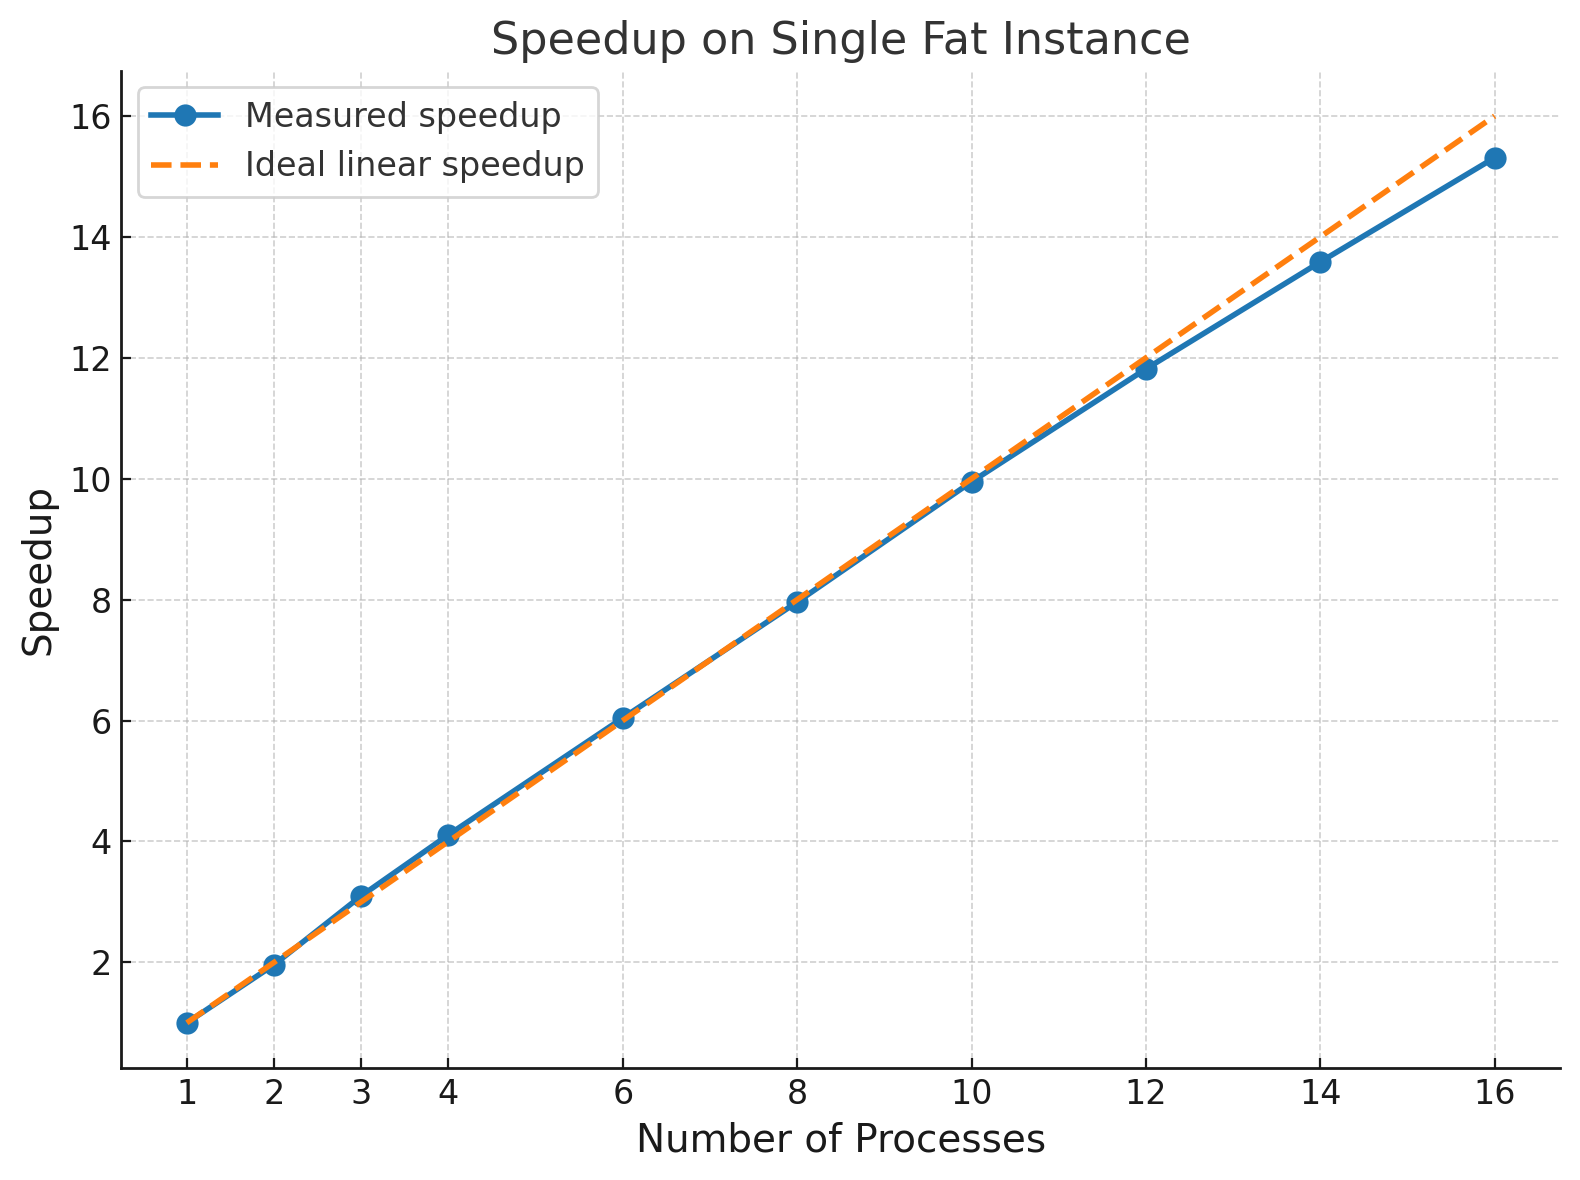
\includegraphics[width=0.5\linewidth]{parallel_strong_scaling_16_cores.png}
\end{frame}

\begin{frame}{Performance Evaluation on GCP (Strong Scaling)}
  \begin{itemize}
    \item Intra-regional clusters: negligible communication overhead.
    \item Inter-regional / multi-region: \texttt{MPI\_Allgatherv} becomes dominant.
  \end{itemize}
  \centering
  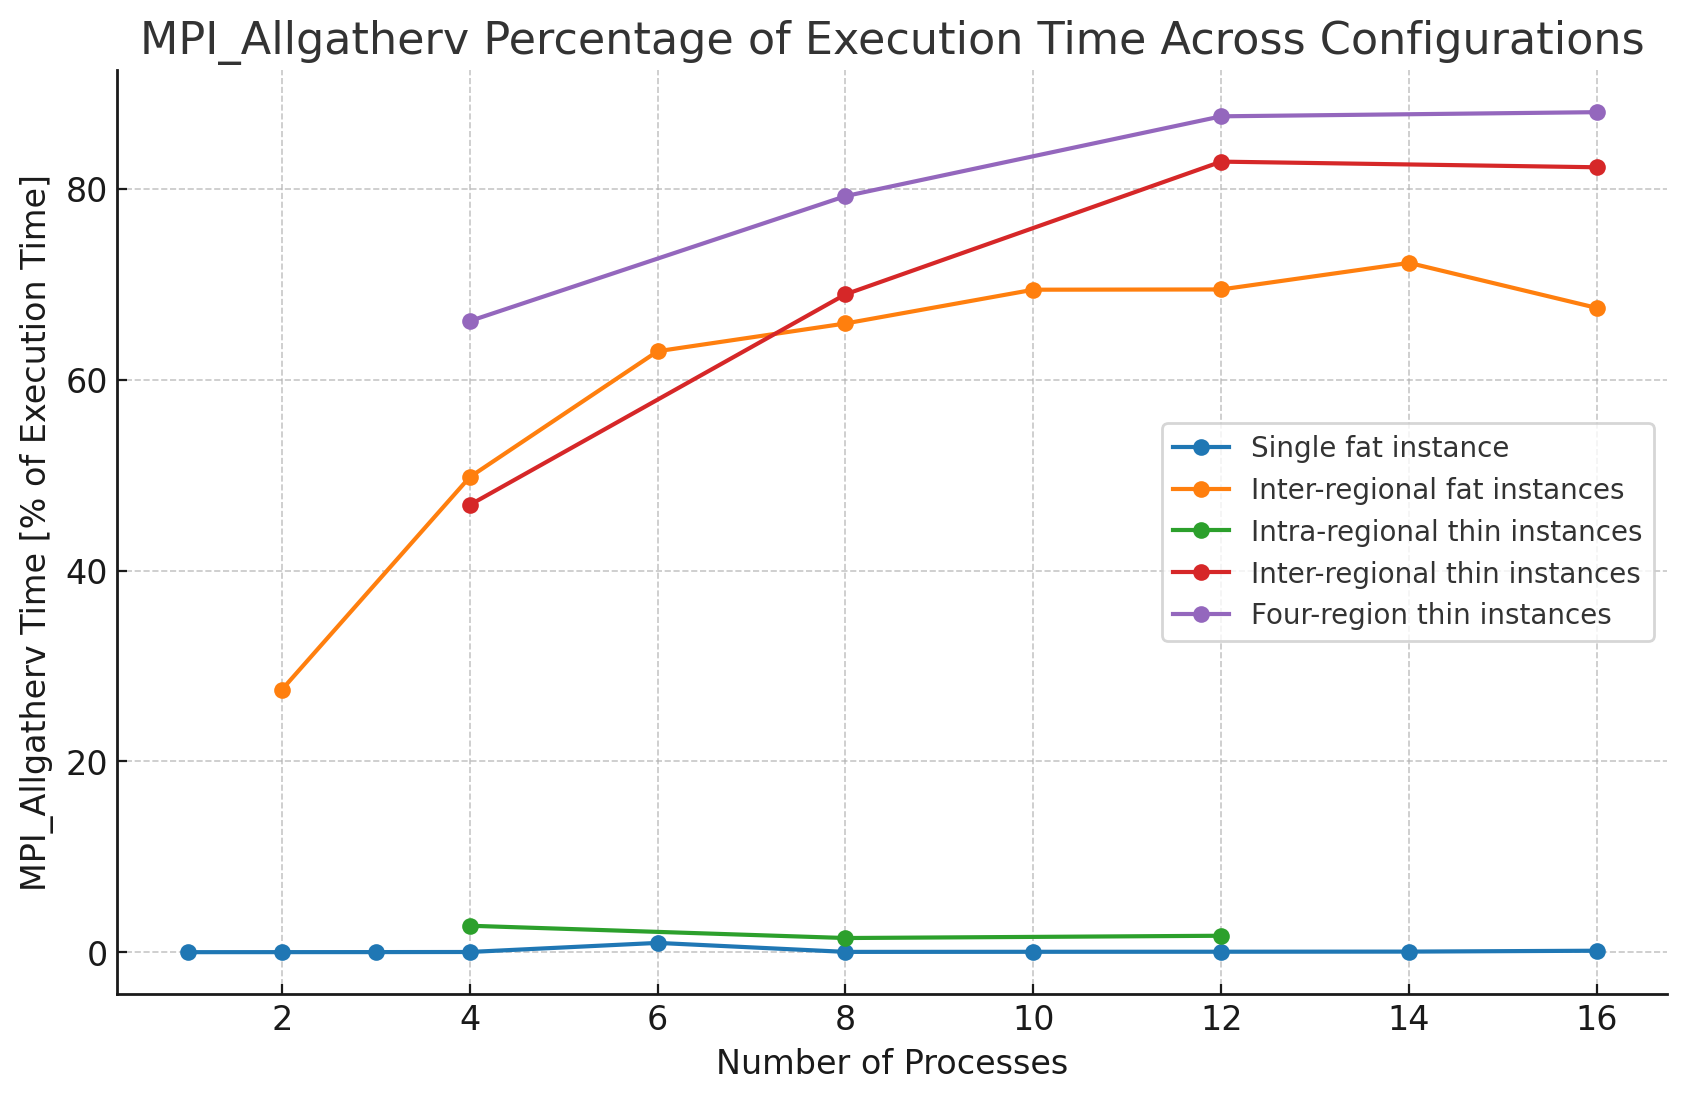
\includegraphics[width=0.85\linewidth]{communication_fraction_ex_time.png}
\end{frame}


\begin{frame}{Performance Evaluation on GCP (Weak Scaling)}
\begin{itemize}
	\item Theoretical weak scalability ($\tfrac{N_p}{P} = N_1$):
\end{itemize}
\[
Scalability(P) = \frac{t_{parallel}(1)}{t_{parallel}(P)} = \frac{N_1^2}{N_p^2}P = \frac{1}{P}
\]
\begin{itemize}
	\item The direct method inherently exhibits poor weak scalability, because each process must still loop over all $N$ bodies when computing accelerations.
\end{itemize}
  \centering
  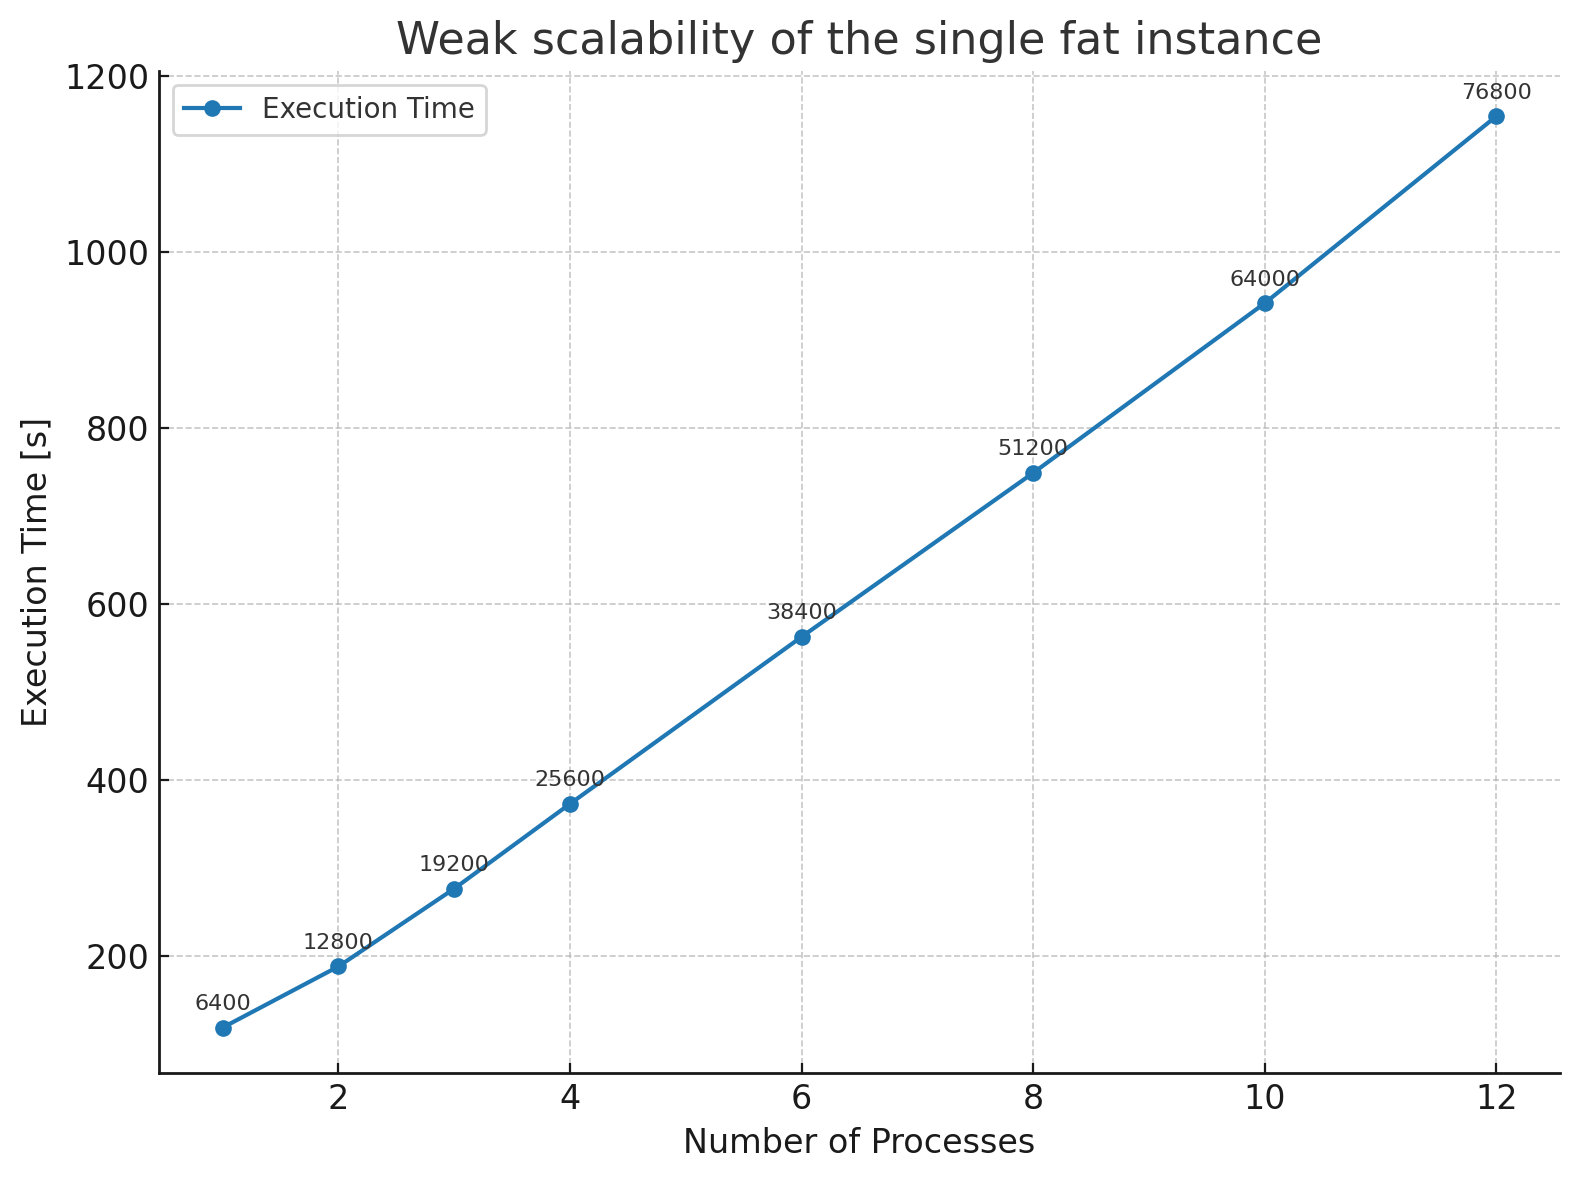
\includegraphics[width=0.47\linewidth]{parallel_weak_scalability.png}
\end{frame}

\begin{frame}{Conclusions}
  \begin{itemize}
    \item Strong scalability holds intra-node / intra-region.
    \item Inter-region latency breaks scalability (blocking collective).
    \item Direct $O(N^2)$ method limits weak scalability.
    \item Future work: hierarchical/approximate methods (e.g., Barnes--Hut).
  \end{itemize}
\end{frame}

\end{document}

